\hypertarget{locomotion}{%
\section{Locomotion}\label{locomotion}}

The word locomotion means ``The act of moving from place to
place.''~\texttt{dictionary} from Latin combining location and motion.
Biology has explored a variety of very interesting ways to move around.
Animals can be carried on currents, swim, crawl, slide, walk, run, jump,
and fly.

Most of the locomotion solutions found in nature are hard to imitate
with machines. Although legs are the base for human locomotion, humans
have valued wheels in their motion solutions. The earliest recorded
appearance of wheels is in Mesopotamia (Sumerian) at the mid-4th
millenium BC. The is evidence of independent discovery in the new world,
the lack of domesticated large animals prevented any development beyond
children's toys.

Rolling is very efficient, especially compared to dragging or carrying
materials. At the macroscopic scale, nature has not developed wheels.
This is not surprising since the wheel needs to be disconnected from the
rest of the system for free rotation reasons, but would then not have
the required nutrient supply (blood or something similar) to grow,
develop and maintain the structure. Although nature did not evolve large
wheels, human motion has some similarities to rolling - a rolling
polygon when motion models are examined.

We are no longer bound to wheels as the only choice for motion. We can
implement a number of nature inspired motion solutions. The type of
motion used by a robot is often the most notable aspect of the machine.
Certainly a great deal of interest and entertainment can be found in
implementing novel locomotion into a robot.

As a robotics engineer, you may be asked to choose the type of motion,
meaning you must choose ``fly, hop, swim, walk, roll ...'' Often the
environment decides for you, for example, if you must operate in the air
or water, or in very rough terrain. You may have other constraints
involved like power consumption, weight or robustness. These constraints
will normally push the design towards one locomotion system.

When looking at a wheel verses an articulator there are some standard
issues that must be addressed. Articulation is much more complicated in
design, control and expense (both energy and financial). Legs
(articulators) require more actuators and thus more control components.
The control system is more complicated than with a wheeled design.
Another consideration is energy. Articulators move their center of mass
for locomotion and may have to move a significant amount of hardware.
Thus there is internal mass movement along with the external mass (the
vehicle). Wheels by their very design keep the center of mass at a
constant distance from the ground. This reduces power usage.

The tradeoff for the efficiency gain is that articulated motion has the
possibility of enhanced environmental robustness. This is clear when
watching any household spider run across a textured ceiling. The most
efficient wheel, the rail wheel is also the least robust in that it does
not operated outside an instrumented environment. Cars use wheels that
can run on a road or flat ground. To go beyond this we need to bring the
rail or road along with - the idea behind tracks. Track systems can
operate in a larger set of environments, but at cost of energy.

\begin{quote}
The relations between energy, speed and motion type.
\end{quote}

\hypertarget{wheels}{%
\section{Wheels}\label{wheels}}

For thousands of years wheels have worked very well. Most vehicles we
imagine are two or four wheeled systems. Two wheels use the gyroscopic
effect to provide stability. Static (passive) stability of the vehicle
is assured by having three wheels and the center of gravity in the
triangle formed by the ground contact points of the wheels. Trikes are
less popular on the road due to concerns about instabilities during
turning. Additional wheels, additional ground contact points, can
improve the stability. Four wheels provides the stability in the turn at
the cost of needing a suspension system (more than three require
suspension). Suspension systems do more than level the ride as they can
keep all the wheels on the ground when traveling over rough terrain.
This provides better traction as well as avoids digging in too deeply.
Larger wheels give greater obstacle traversal due to the decreased angle
of attack which reduces the required torque. Bigger wheels are heavier
and require greater reductions in the gear box however. Selection of
wheels is based on the surface and the application. Hard dry smooth
surfaces may use smooth wheels and rougher or slicker surfaces demand
tires that are rough and maybe soft.

The effectiveness of the wheel is given by the contact area of the
wheel. This is a combination of wheel width and tread design. Angle of
contact combined with tire shape will affect the steering response.
Wheel tread, width and other parameters will affect the rolling friction
and the energy loss in motion. To gain maneuverability, wheels can be
steered or replaced with omni-wheels. This requires additional hardware
and controls which increases complexity, weight and cost. Most designs
do not allow the craft to maneuver and orient simultaneously and
independently which increases the control effort. As with many aspects
of engineering, this is a tradeoff between simple, robust and
inexpensive design verses a flexible, maneuverable, adaptable design.

\hypertarget{omni-mecanum-and-spherical-wheels}{%
\subsection{Omni, Mecanum and Spherical
Wheels}\label{omni-mecanum-and-spherical-wheels}}

Of all the wheel types, none captures attention like the omni and
Mecanum wheels. Their operation is unexpected and at first seems to defy
intuition. These wheels are capable of motion in the rolling direction
as well as motion along the axle direction which leads to holonomic
robots. Which means the robot can position and orient independently in
the plane. It makes for a very maneuverable robot which is very popular.
These wheels require hard flat surfaces to work properly. If the dirt or
small stones get lodged into the rollers or if the rollers lose contact
with the surface, the holonomic motion is compromised. So these wheels
are used exclusively indoors. Since fine precision maneuvering is
normally required for indoor systems and not outdoor systems, there has
not been much effort expended to make outdoor versions.

\begin{quote}
The Airtrax forklift.

The Airtrax scissor lift.
\end{quote}

The omni wheel's first patent was in 1919 by Grabowiecki. The Mecanum
wheel was developed by Bengt Erland Ilon in 1972 while working for the
Mecanum company. Airtrax, an American forklift company purchased patent
rights and briefly manufactured forklifts with a heavy duty version of
the Mecanum wheel. These wheels have much less ground friction in a turn
in comparison to a skid steer requiring much less torque.

\begin{quote}
The \(\gamma\) measure.

The (a) \(\gamma = 0\) configuration and (b) \(\gamma = 45^\circ\)
configuration.
\end{quote}

For this text, we will combine the omni and Mecanum wheels and just call
them omniwheels. The difference between them is only in the angle the
rollers are mounted on the wheel body. \texttt{gammaconfig} shows some
sample types of omniwheels using the \(\gamma = 0\) configuration and
\(\gamma = 45^\circ\) configuration. Normally the \(\gamma=0\) style of
wheel is used in non-parallel mounting as shown in the first robot in
the \texttt{gammawheelmounting} and the parallel mounting is used for
the other standard type of wheel design using \(\gamma = 45^\circ\).

\begin{quote}
Normal mounting style for \(\gamma = 0\) and \(\gamma = 45^\circ\).

Force vectors induced by rotation with the \(\gamma = 45^\circ\)
configuration. This is the view from the ground.

Mecanum rotation directions and vector forces for different vehicle
directions.

Summary of wheel motion and directions
\end{quote}

\begin{itemize}
\tightlist
\item
  Driving forward: all four wheels forward
\item
  Driving backward: all four wheels backward
\item
  Driving left: 1,4 backwards; 2,3 forward
\item
  Driving right: 1,4 forward; 2,3 backward
\item
  Turning clockwise: 1,3 forward; 2,4 backward
\item
  Turning counterclockwise: 1,3 backward; 2,4 forward
\end{itemize}

Note that if you swap front and back wheel orientation you will see that
left/right motion will get flipped. The convention for this text will be
that the rollers contact the ground in the orientation shown in Figure
\texttt{meccanumwheelvectors}, meaning

A variation of the omni wheel is the omni ball developed by Kaneko
Higashimori Lab at Osaka University, see~\texttt{fig:omniball}. This
wheel will be used to drive tracks in a very novel approach described in
the tracks section below. This wheel fails to be a true spherical wheel
as far as two directional motion is concerned and has motion equations
similar to the omniwheel systems.

\begin{quote}
The Omni Ball Wheel developed at the Kaneko Higashimori Lab at Osaka
University
\end{quote}

Omni and Mecanum wheels can be driven on only one direction and only
when combined with other wheels are they able to move against the
rolling directions. To gain two dimensional directional capability the
wheel needs to be a sphere or at least approximate the sphere in a
significant manner. This can be done by reversing the power direction
from the classical mechanical computer mouse. In the mechanical mouse
the ball is forced around which drives small disks inside in the
component directions. By mounting three omniwheels on top of a ball, one
can gain motion in two directions. \texttt{fig:robotonball} shows one
design by Dr. Masaaki Kumagai, director of the Robot Development
Engineering Laboratory at Tohoku Gakuin University.

\begin{figure}
\centering
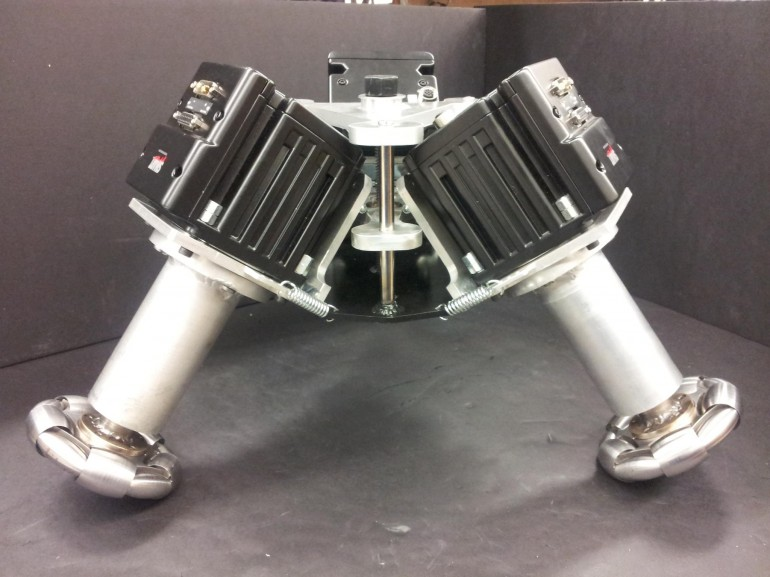
\includegraphics[width=0.6\textwidth,height=\textheight]{MotionFigures/sds-omni-1.jpg}
\caption{Omniwheel drive system}
\end{figure}

Omniwheel balancing robot

\begin{figure}
\centering
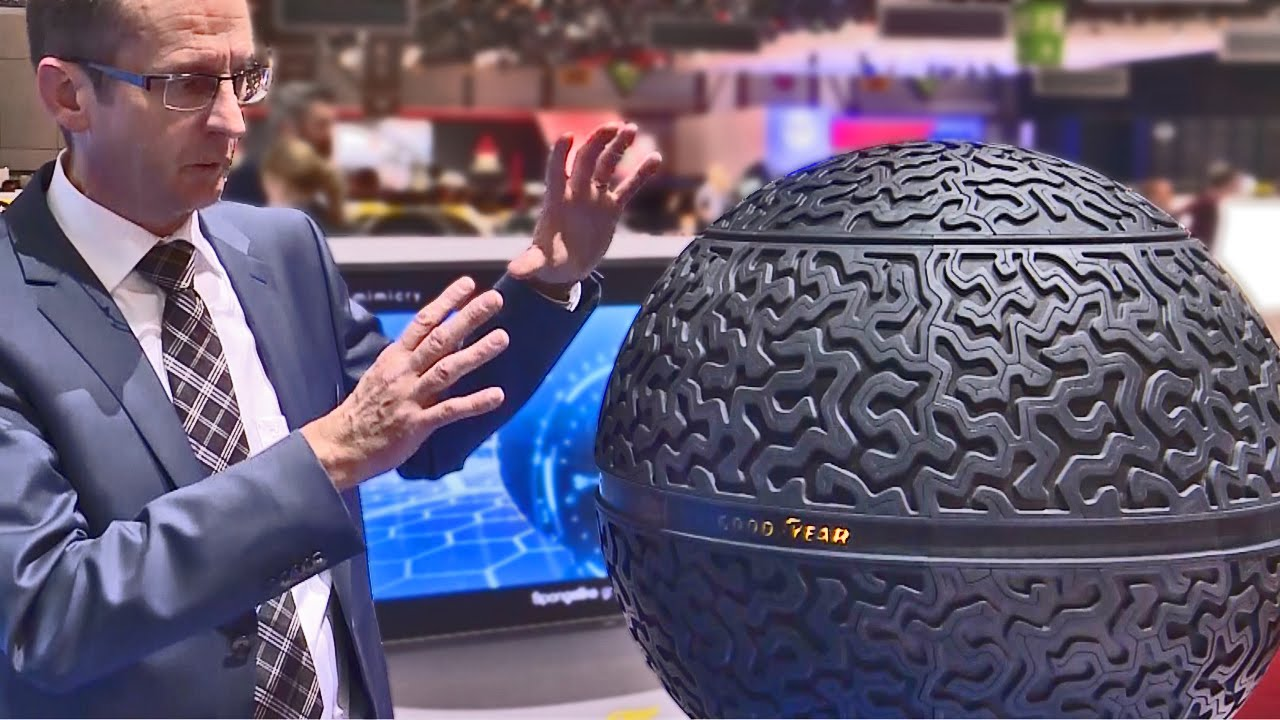
\includegraphics[width=0.6\textwidth,height=\textheight]{MotionFigures/goodyearsphere.jpg}
\caption{GoodYear Spherical Wheel Concept Tire}
\end{figure}

\begin{figure}
\centering
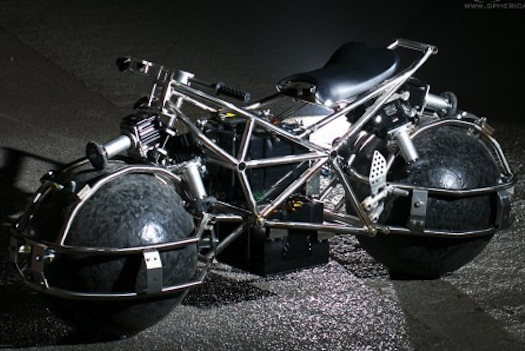
\includegraphics[width=0.6\textwidth,height=\textheight]{MotionFigures/SDS-omnidirectional-electric-motorcycle4.jpg}
\caption{Prototype omnidirectional motorcycle}
\end{figure}

\hypertarget{mobility-issues}{%
\subsection{Mobility Issues}\label{mobility-issues}}

The stability of the craft is given by several factors. Having less than
three contact points requires dynamic balance for a system which is ``at
rest''. Having less than 6 contact points means that during locomotion,
the system requires dynamic balance during motion or one is moving at
most two legs at a time making a more complicated control system. The
location of the center of gravity is an important aspect of dynamic
stability. A lower center of gravity helps to avoid falling over.

For ground systems, the terrain will have more influence than with air
or sea. We have to worry about the terrain roughness, slickness, grades
and other issues. The number of wheels, type of wheels, type of
suspension, and steering will all have a large affect on the
effectiveness of motion.

\hypertarget{tracks}{%
\subsection{Tracks}\label{tracks}}

For the purposes of this text, we will treat unsteered tracked systems
(tank treads) as two-wheel differential drive (wheeled) systems. The
modeling is more difficult than with wheels. Modeling the skid-steer
turns requires details about the track system and the surface. Since
rocks, mud and other aspects of the surface can have significant effects
on turning friction, models have limited utility.

\hypertarget{legs}{%
\section{Legs}\label{legs}}

We now move over to a more biological approach. The use of legs in
locomotion has been very successful. Animals range in sizes from single
millimeter to multiple meter range. Legs have proved invaluable at many
space and speed dimensions. In the robotics view, a leg is articulated
manipulator (serial chain). This means that it requires many of the same
controls that a robot arm would require, but adapted to the specific
task of moving the robot. Although a hobby level robot can implement 6
simple articulators to produce insect like motion, getting natural,
efficient, robust and fast bipedal and quadrupedal motion is very
difficult.

\hypertarget{aspects-of-articulated-based-motion}{%
\subsection{Aspects of Articulated Based
Motion}\label{aspects-of-articulated-based-motion}}

Engineers are experimenting with 2 - 8 leg designs to learn more about
articulator locomotion as well as what it can teach us about the animals
that have similar designs. We know that for static stability, at least
three points of contact are required. So, three legs are required to
stand still. When we move, some of the legs must move forward to
initiate the gait. If we want three points on the ground, this means six
legs is the minimum for stable walking. Robots using six or more legs do
not need a balance control system.

Systems using four legs have a static balance when still, but must use a
dynamic control approach to maintain balance during the step. This is a
variation of the inverted pendulum problem which is discussed in the
chapter on motion control. Finally our system of using two legs requires
a control system for moving and standing.

\begin{figure}
\centering
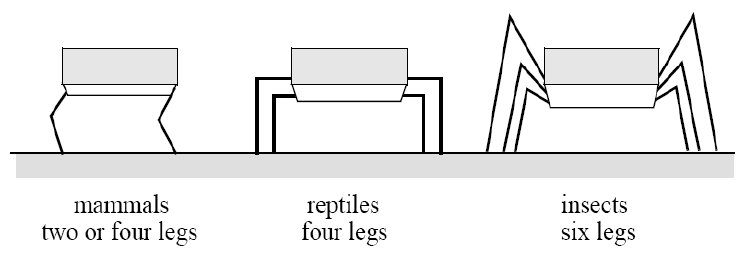
\includegraphics[width=0.5\textwidth,height=\textheight]{MotionFigures/legs.png}
\caption{}
\end{figure}

Increasing the number of legs will increase weight, power requirements,
coordination problems and control hardware. Adding legs, as mentioned
before, will help with stability and provide a greater number of contact
points. Increasing ground contact can increase traction and robustness,
depending on the contact area, angle of contact, friction, surface
roughness and friction. For static stability we want the center of mass
to fall inside the span of the legs. Unlike wheels, the center of mass
for a leg moves up and down as the robot walks. This decreases power
efficiency, increases the chance of a shifting center of gravity which
makes path planing more difficult. In complicated environments, one may
have to plan the motion of each articulator. The configuration space for
a 6 legged robot with three servos is 18, which is rather large for path
planning and might fail due to size.

\begin{figure}
\centering
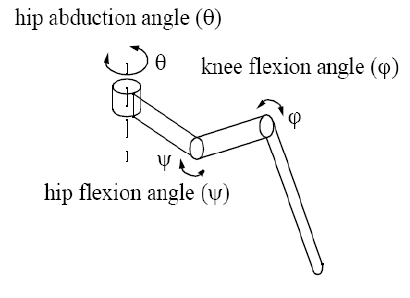
\includegraphics[width=0.5\textwidth,height=\textheight]{MotionFigures/legjoint.png}
\caption{Leg joints and their use.}
\end{figure}

\begin{itemize}
\item
  Two DOF is required:\\
  lift and swing
\item
  Three DOF is needed in most cases:\\
  lift, swing and position
\item
  Fourth DOF is needed for stability:\\
  ankle joint - improves balance and walking
\end{itemize}

Consider a humanoid robot. How complex are they? A leg has a hip (two
degrees of freedom) and knee plus ankle which gives another two degrees
of freedom. So a leg is a 4 DOF (degrees of freedom) structure. An arm
is at least 5 DOF. A head has pan and tilt so at least 2 DOF. This adds
up to 20 DOF for a humanoid style robot. Motion planning and control is
challenging for high DOF robots. Good tools for doing this is an active
area of research.

\begin{figure}
\centering
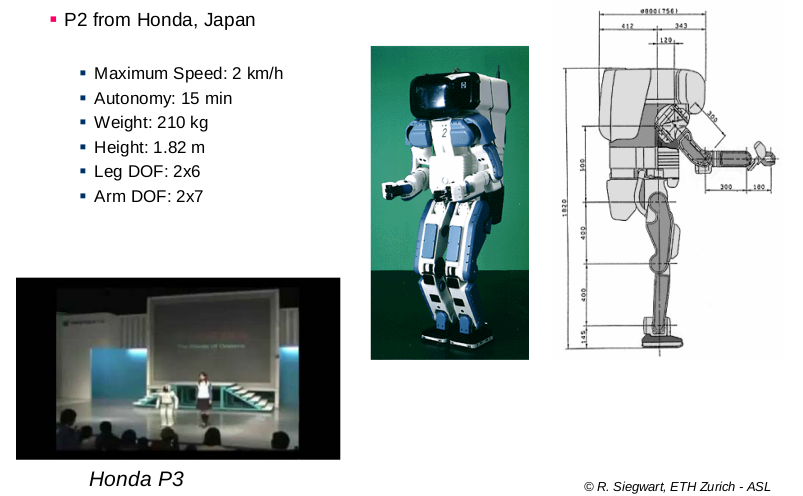
\includegraphics{MotionFigures/humanoid.png}
\caption{}
\end{figure}

There are several attempts to combine legs and wheels. The Shrimp is one
such design, \texttt{shrimp}. Many fun and interesting innovations come
from the suspension system. Adaptive (passive or active) suspension is a
current area of development, \texttt{adaptivesuspension}. Other lines of
development look to blending sensing with the wheel or suspension
system. One example is the flexible wheel, \texttt{flexiwheel}.

\begin{quote}
Walking Wheels

Adaptive Suspension

Flexible Wheel
\end{quote}
